\documentclass[11pt,titlepage,twoside]{article}
\usepackage{geometry}                % See geometry.pdf to learn the layout options. There are lots.
\geometry{letterpaper}                   % ... or a4paper or a5paper or ... 
%\geometry{landscape}                % Activate for for rotated page geometry
%\usepackage[parfill]{parskip}    % Activate to begin paragraphs with an empty line rather than an indent
\usepackage{graphicx}
\usepackage{amssymb}
\usepackage{epstopdf}
\usepackage{url}
\usepackage{hyperref}
\usepackage{fancyhdr}
%\DeclareGraphicsRule{.tif}{png}{.png}{`convert #1 `dirname #1`/`basename #1 .tif`.png}

\def\ProgramVersionNoSpace{{VERSION}}
\def\ProgramVersion{{\ProgramVersionNoSpace \space}}
\def\ImagePath{{images}}

\title{PSF Estimator \ProgramVersion User Guide}
\author{Cory Quammen}
%\date{}                                           % Activate to display a given date or no date

\usepackage{fancyhdr}
\setlength{\headheight}{15pt}
 
\pagestyle{fancy}
 
\fancyhf{}
\fancyhead[LE,RO]{\thepage}
\fancyhead[RE]{\textit{PSF Estimator \ProgramVersion User Guide}}
\fancyhead[LO]{\textit{\nouppercase{\leftmark}}}
 
\fancypagestyle{plain}{ %
\fancyhf{} % remove everything
\renewcommand{\headrulewidth}{0pt} % remove lines as well
\renewcommand{\footrulewidth}{0pt}}

\begin{document}
\maketitle
\tableofcontents
\vfill

\pagebreak

\section{Introduction}

PSF Estimator is a program for computing a noise-free estimate of a point-spread function (PSF) of widefield and confocal microscopes. It works by fitting an analytical model of the \emph{bead-spread function} to an image of a sub-diffraction-limit-sized fluorescent bead. The bead-spread function (BSF) is calculated as the convolution of the PSF with a sphere whose radius is the same as the radius of the physical bead used to produce the measured image.

The fitting process minimizes the mean squared difference between pixels in the measured image and corresponding pixels in the calculated image. This process yields a maximum likelihood estimate of the PSF (assuming that noise is Gaussian distributed).

\subsection{System Requirements}

PSF Estimator \ProgramVersion requires Windows XP, Windows 7, or Macintosh OS X 10.5 or higher running on an Intel processor. A recent graphics card is recommended.

Your system should have at least 150 MB of hard drive space free to install the program. At least 512 MB of RAM is required, but 2 GB is recommended.

\subsection{Acknowledgements}

PSF Estimator \ProgramVersion is developed and maintained by the \href{http://www.cismm.org}{Center for Computer Integrated Systems for Microscopy and Manipulation}, a \href{http://www.nibib.nih.gov/}{National Institute of Biomedical Imaging and Bioengineering Resource}, award number P41-EB002025. Additional work was supported by the National Library of Medicine Insight Toolkit Adapters, Algorithms, Data, and Distribution program.

\section{Installation}

Installation of PSF Estimator \ProgramVersion is similar to installation of any other program.

\subsection{Getting the software}

To obtain the latest installer for PSF Estimator \ProgramVersionNoSpace, visit \url{http://www.cismm.org/downloads}. Please choose either the Mac or Windows version of the program, whichever is suitable for your system.

Source code for the program is also available there in the form of a Git repository, enabling you full access to the algorithms used to generate the images and providing the opportunity to submit bug fixes back to the project. 

\subsection{Windows installation}

Double-click the setup program named \textbf{PSFEstimator-\ProgramVersionNoSpace-win32.exe}. On the first screen, click \emph{Next}. Please read the program license. If you agree to the terms of the license, click \emph{I Agree}. On the next screen, choose where you want to install the program. The default directory is the most-used option. Click \emph{Next}. You may optionally choose a different location in the Start Menu. By default, it will be placed in the CISMM folder. Click \emph{Install}.

\subsection{Mac installation}

Double-click the Macintosh disk image named \textbf{PSFEstimator-\ProgramVersionNoSpace-darwin.dmg}. An installer program will launch and ask you to agree to the terms of the license. If you agree, a disk image named \textbf{PSFEstimator-\ProgramVersionNoSpace-Darwin} will appear on your desktop and a new Finder window will open.

To install the program in your \emph{Applications} directory on your computer's hard drive, drag the PSF Estimator \ProgramVersion application to either the \emph{Applications} alias in the Finder window that just appeared or drag it directly to your \emph{Applications} directory.

\subsection{Running the program}

\subsubsection{Windows}

You can launch the PSF Estimator program from the Start menu. If you chose the default installation location and menu folder, select \emph{Start} $\rightarrow$ \emph{All Programs} $\rightarrow$ \emph{PSF Estimator \ProgramVersionNoSpace} $\rightarrow$ \emph{PSF Estimator \ProgramVersionNoSpace}.

\subsubsection{Macintosh}

If you installed the application in the \emph{Applications} directory on your hard drive, double-click the program \emph{PSF Estimator \ProgramVersionNoSpace}.

\subsection{Where to get help}

If you have trouble installing or running the program or have questions about its usage, please please contact  \href{mailto:cquammen@cs.unc.edu}{Cory Quammen $\langle$cquammen@cs.unc.edu$\rangle$}. Unfortunately, no guarantee of support can be provided, but we will do our best to help you solve your problem.

\section{Getting to know PSF Estimator}

This section gives a tour of the many features in PSF Estimator.

\subsection{Program Window}

\begin{figure}[h]
  \centering
  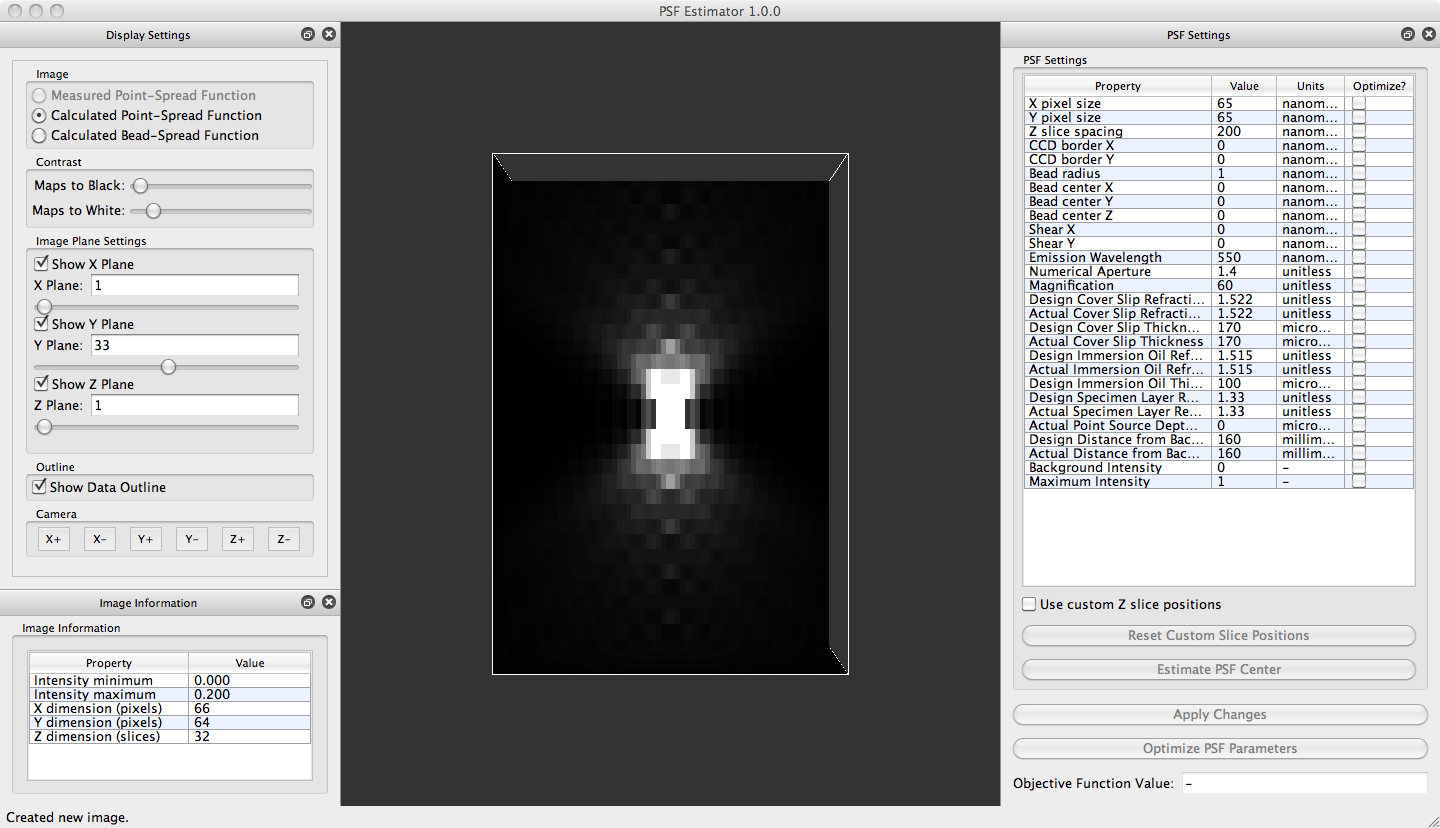
\includegraphics[scale=0.3]{\ImagePath/ProgramWindow}
  \caption{The PSF Estimator program window.}
  \label{fig:ProgramWindow}
\end{figure}

The main program window is organized into several sections. 

\subsubsection{Visualization Panel}

The \emph{Visualization Panel} (center, Figure \ref{fig:ProgramWindow}) displays PSFs via three orthogonal cutting planes. A measured PSF imported into the program, a calculated PSF, or a calculated bead-spread function (BSF, the image of a spherical bead convolved with the PSF) can be displayed here. Only one of these images may displayed at one time; switching between them enables visual inspection of the PSF fitting results.

\subsubsection{Display Settings}

The \emph{Display Settings} control which PSF image is displayed in the \emph{Visualization Panel} and how it is displayed.

\begin{description}

  \item[Image] \hfill
   \begin{figure}[h]
    \centering
    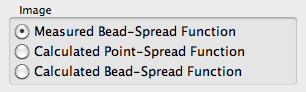
\includegraphics[scale=0.5]{\ImagePath/ImageControls}
    \caption{The image controls determine which image is displayed in the \emph{Visualization Panel}.}
    \label{fig:ImageControls}
  \end{figure}
 
The controls shown in Figure \ref{fig:ImageControls} let you choose which image to display: the measured bead-spread function, the point-spread function corresponding to the current PSF settings, the bead-spread function corresponding to the current PSF settings, or the difference between the measured image and the bead-spread function. If no measured image is loaded in the program, then the \emph{Measured Bead-Spread Function} and \emph{Measured Minus Calculated BSF} are disabled.

  \item[Contrast] \hfill \\
  
    \begin{figure}[h]
    \centering
    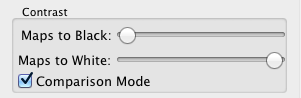
\includegraphics[scale=0.5]{\ImagePath/ContrastControls}
    \caption{Contrast controls.}
    \label{fig:ContrastControls}
  \end{figure}
  
  The contrast controls (Figure \ref{fig:ContrastControls}) determine which PSF/BSF image voxel value maps to black and which voxel value maps to white. The range of the controls is set to the minimum and maximum voxel values in the image selected in the \emph{Image} panel.

  \item[Image Plane Settings] \hfill \\
  
    \begin{figure}[h]
    \centering
    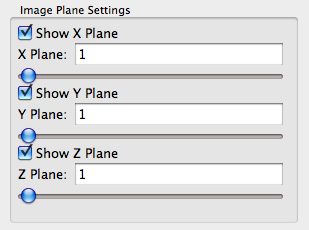
\includegraphics[scale=0.5]{\ImagePath/ImagePlaneSettingsControls}
    \caption{Image plane settings controls.}
    \label{fig:ImagePlaneSettingsControls}
  \end{figure}
  
  Shown in Figure \ref{fig:ImagePlaneSettingsControls}, these controls determine which slices through the image in the $yz$, $xz$, and $xy$ planes are displayed and whether those image planes are displayed. The range for the \emph{X Plane} setting is from 1 to the number of voxels into the $x$-direction, and the range for the \emph{Y Plane} and \emph{Z Plane} are similarly defined.

  \item[Outline] \hfill \\
  
  \begin{figure}[h]
    \centering
    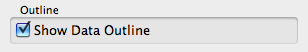
\includegraphics[scale=0.5]{\ImagePath/OutlineControls}
    \caption{Outline controls.}
    \label{fig:OutlineControls}
  \end{figure}
  
  
  This control enables you to display or hide an outline of the image data.

  \item[Camera] \hfill \\
  
  \begin{figure}[h]
    \centering
    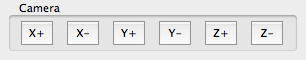
\includegraphics[scale=0.5]{\ImagePath/CameraControls}
    \caption{Camera controls.}
    \label{fig:CameraControls}
  \end{figure}
  
  These controls consist of six buttons that move the camera to six canonical positions. The +X button moves the camera to look down the positive $x$-axis and the -X button move the camera to look down the negative $x$-axis. The $-Y$, $+Y$, $-Z$, and $+Z$ have similar functions, but operate on different coordinate axes.

\end{description}

\subsubsection{Image Information}

  \begin{figure}[h]
    \centering
    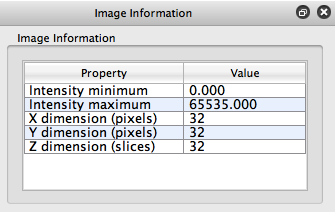
\includegraphics[scale=0.5]{\ImagePath/ImageInformationControlPanel}
    \caption{Image information control panel.}
    \label{fig:ImageInformationControlPanel}
  \end{figure}


The \emph{Image Information} control panel displays information about the image currently displayed in the \emph{Visualization Panel}. Information includes the minimum and maximum voxel intensity of the image and the size of the image in the $X$-, $Y$-, and $Z$-dimensions.

\subsubsection{PSF Settings}

\begin{figure}[h]
  \centering
  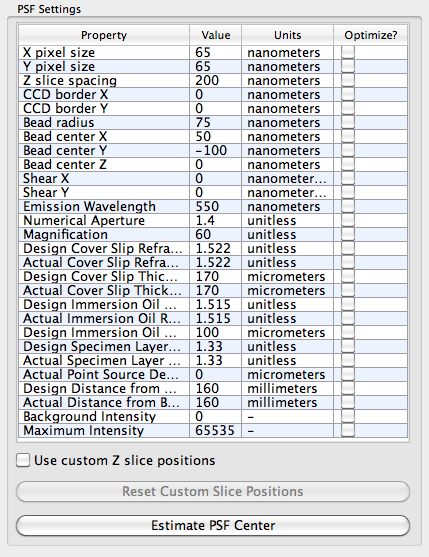
\includegraphics[scale=0.5]{\ImagePath/PSFSettingsControlPanel}
  \caption{PSF settings control panel.}
  \label{fig:PSFSettingsControlPanel}
\end{figure}

The PSF settings table is used to set parameters for the analytical PSF and BSF models. The table has four columns giving the parameter name, parameter value, unit of measurement of the parameter, and a checkbox indicating whether the parameter will be optimized. Descriptions of individual parameters for PSF models supported by the program are described in Section \ref{sec:PointSpreadFunctionSettings} of this manual.

The remaining controls are described below.

\begin{description}

  \item[Custom Z slice positions] \hfill \\
  
When checked, the \emph{Use custom Z slice positions} checkbox adds one PSF parameter in the PSF settings table for each Z slice in the image. This feature can be used to fit image stacks obtained on microscopes with motorized stages that do not produce a uniform Z spacing at nanometer accuracy.

  \item[Reset Custom Slice Positions] \hfill \\
  
When clicked, this button resets the custom Z slice position parameters in the PSF settings table to be evenly spaced with the spacing determined by the \emph{Z slice spacing} parameter. The center of the image along the Z dimension is defined to be at position Z = 0. This button is enabled only when the \emph{Custom Z slice positions} option is checked.

  \item[Estimate PSF Center] \hfill \\
  
Clicking this button sets the center of the BSF to the center of the voxel with highest intensity in the measured BSF image.

  \item[Apply Changes] \hfill \\
  
  Because the computation of the BSF may take several seconds, the BSF image is not updated as soon as a parameter value is changed. Instead, the BSF is updated when the \emph{Apply Changes} button is clicked. This button is enabled only after a parameter has changed.
  
  \item[Optimize PSF Parameters] \hfill \\
  
  This button starts an optimization routine that searches for parameter values that minimize an objective function. Only parameters selected for optimization (those whose checkbox in the \emph{Optimize?} column of the PSF settings table is checked) are modified by the optimization routine. Optimizing a few parameters is faster than optimizing numerous parameters.
  
  \item[Objective Function Value] \hfill \\
  
  This displays the value of the objective function used for model fitting. Lower numbers are better.

\end{description}




\subsection{Menu Bar}

The menu bar in PSF Estimator contains three menus that provide various commands. Each menu is described in more detail below.

\subsubsection{File Menu}

The \emph{File Menu} features options for creating PSFs of arbitrary size, opening images, saving PSF images, and loading and saving program sessions.

\begin{description}
  \item[New Image] \hfill \\
  Creates a new PSF with default settings. The size and voxel spacing of the new image are set prior to the creation of the image. This option is useful for generating a theoretical PSF at arbitrary voxel size when the PSF parameters are known.

  \item[Open Image...] \hfill \\
  Opens image data. 3D TIFF, VTK, and LSM files are supported. Sequences of 2D TIFF images currently cannot be imported.

  \item[Save PSF Image...] \hfill \\
   Saves the point-spread function image to a file. The image can be exported as a 3D TIFF, VTK, or LSM image.
   
  \item[Save BSF Image...] \hfill \\
  Saves the bead-spread function image to a file. The image can be exported as a 3D TIFF, VTK, or LSM image.
  
  \item[Load Session...] \hfill \\
  Loads the program session file that contains all the program settings from a previous session. This option enables you to do some work in PSF Estimator, save some work, restart the program, and continue where you left off.
  
  \item[Save Session...] \hfill \\
  Save the program session file that contains all the current program settings.
  
  \item[Exit] \hfill \\
  Exits the program. \textbf{Macintosh users:} The \emph{Quit} menu item appears under the \emph{PSFEstimator} menu instead of the \emph{File} menu.

\end{description}
\subsubsection{Edit Menu}

\begin{description}

  \item[Copy] \hfill \\
  Copies text in a text field.
  
  \item[Paste] \hfill \\
  Pastes text into a text field.
  
\end{description}

\subsubsection{Window Menu}

\begin{description}

  \item[About PSFEstimator] \hfill \\
  Shows a window with information about PSF Estimator. \textbf{Macintosh users:} The \emph{About PSFEstimator} menu item appears under the \emph{PSFEstimator} menu instead of the \emph{Window} menu. 

  \item[Display Window] \hfill \\
  Shows/hides the \emph{Display Settings Control Panel}. If you close the \emph{Display Settings Control Panel}, you can show it again with this menu item.
  
  \item[Image Information] \hfill \\
    Shows/hides the \emph{Image Information Control Panel}. If you close the \emph{Image Information Control Panel}, you can show it again with this menu item.
  
  \item[PSF Settings] \hfill \\
  Shows/hides a separate panel that displays the fluorescence images simulated by FluoroSim.

\end{description}

\section{Point-Spread Function Settings}
\label{sec:PointSpreadFunctionSettings}

\subsection{Gibson-Lanni PSF Model for Widefield Microscopes}

\begin{description}

  \item[X pixel size] \hfill \\
   The physical size of the pixel in the $x$ direction.
  
  \item[Y pixel size] \hfill \\
   The physical size of the pixel in the $y$ direction.
  
  \item[Z slice spacing] \hfill \\
   The spacing between slices in the images.
  
  \item[Bead radius] \hfill \\
   The radius of the spherical bead used to generate the measured BSF images.
  
  \item[Bead center X] \hfill \\
   The position of the bead center in the $x$ direction. The origin is defined to be the center of the measured BSF image.
  
  \item[Bead center Y] \hfill \\
   The position of the bead center in the $y$ direction. The origin is defined to be the center of the measured BSF image.
  
  \item[Bead center Z] \hfill \\
   The position of the bead center in the $z$ direction. The origin is defined to be the center of the measured BSF image.
    
  \item[Shear X] \hfill \\
Models lateral stage movement in the $x$-direction as a linear function directly proportional to the $z$-depth of the focal plane. The $x$-offset in the shear direction is defined as
\begin{equation}
x_{\mathrm{offset}} = m_{x} z
\end{equation}
where $m_{x}$ is the \emph{Shear in X} setting value and $z$ is the focal plane depth. The $x_{\mathrm{offset}}$ is added to the $x$-coordinate of each voxel position during image generation.

  \item[Shear Y] \hfill \\
   Same as \emph{Shear in X} but in the $y$-direction.

  \item[Emission Wavelength] \hfill \\
   The dominant wavelength in the emission spectrum from the fluorophores in the fluorescently labeled bead.
  
  \item[Numerical Aperture] \hfill \\
   The numerical aperture of the microscope objective lens.
  
  \item[Magnification] \hfill \\
   The magnification of the microscope objective lens.

  \item[Design Cover Slip Refractive Index] \hfill \\
   The cover slip refractive index for which the objective lens was designed.
  
  \item[Actual Cover Slip Refractive Index] \hfill \\
   The actual cover slip refractive index used in the setup for imaging the bead.
  
  \item[Design Cover Slip Thickness] \hfill \\
   The cover slip thickness for which the objective lens was designed.
  
  \item[Actual Cover Slip Thickness] \hfill \\
   The actual cover slip thickness used in the setup for imaging the bead.
  
  \item[Design Immersion Oil Refractive Index] \hfill \\
   The immersion oil refractive index for which the objective lens was designed.
  
  \item[Actual Immersion Oil Refractive Index] \hfill \\
   The actual immersion oil refractive index used in the setup for imaging the bead.
  
  \item[Design Immersion Oil Thickness] \hfill \\
   The immersion oil thickness for which the objective lens was designed.
  
  \item[Design Specimen Layer Refractive Index] \hfill \\
   The specimen layer refractive index for which the objective function was designed. The specimen layer lays below the cover slip.
  
  \item[Actual Specimen Layer Refractive Index] \hfill \\
   The actual specimen layer refractive index in the setup for imaging the bead.
  
  \item[Actual Point Source Depth in Specimen Layer] \hfill \\
   The depth of the specimen below the coverslip.
  
  \item[Design Distance from Back Focal Plane to Detector] \hfill \\
   The design distance from the back focal plane of the objective lens to the CCD camera.
  
  \item[Actual Distance from Back Focal Plane to Detector] \hfill \\
   The actual distance from the back focal plane of the objective lens to the CCD camera.
  
  \item[Intensity Shift] \hfill \\
   A uniform background intensity added to each voxel intensity value. This value is added to the image before the \emph{Intensity Scale} parameter is applied. The parameter value is typically found via optimization.
  
  \item[Intensity Scale] \hfill \\
   This parameter is a scale factor for each voxel intensity. Each voxel intensity is multiplied by this value after the \emph{Intensity Shift} value is added to it. The parameter value is typically found via optimization.
 
\end{description}

\subsection{Gaussian PSF Model for Confocal Microscopes}

A Gaussian PSF model suitable for confocal microscope PSF estimation will be available in a future version of the PSF Estimator.

\section{Using PSF Estimator}

This section provides some helpful tips for using the program.

\subsection{Preparing Data}

PSF Estimator loads only single files representing a 3D image. Unfortunately, sequences of 2D images cannot be loaded. ImageJ can be used to convert just about any image used in microscopy to a 3D TIF image suitable for importing into PSF Estimator.

\subsection{Locating a Suitable Bead in an Image}

Depending on your protocol for imaging sub-diffraction-limited beads to obtain a point-spread function, your 3D image of fluorescent beads may have numerous beads in the field of view. For performance reasons, you'll want to crop the full 3D image in the X and Y dimensions, but do not crop in Z; you will want as much out-of-focus information as you can get. The cropped region should be sufficiently large to ensure that the full extent of the PSF (wherever the intensities are above the mean background intensity) is retained. Since PSF Estimator is designed to fit the PSF to an image of a single bead, it is important to crop out a region of a bead that is well-separated from neighboring beads. PSF Estimator does not have a feature to crop images, so an external image tool is required for this step. ImageJ can crop 3D images easily.

\subsection{Importing the Image}

Select the \emph{Open Image...} item in the \emph{File} menu. In the file chooser that appears, select the bead image you wish to load.

\subsection{Setting Initial Parameters}

It is likely that you know values for some of the parameters, such as \emph{X pixel size}, \emph{Y pixel size}, and \emph{Z slice spacing}. Set the values you know in the PSF settings table. Depending on the PSF model you are fitting, you may know other parameter values as well. Examples include \emph{Numerical Aperture} and \emph{Design Cover Slip Refractive Index} in the Gibson-Lanni PSF model. Set these values according to what you know about the microscope.

Click the \emph{Estimate PSF Center} button to estimate the bead center parameters.

\subsection{Optimization}

Fitting the PSF to the imported bead image involves an optimization process. Experience has shown that performing several separate optimizations is helpful for obtaining a good PSF fit quickly. These sub-optimizations are described below.

\subsubsection{Optimize Intensity Shift and Intensity Scale}

These parameters are perhaps the most important parameters to estimate accurately. They modify the voxel intensities via a linear transform to match the intensity range of the measured image. Assuming the bead center is close to the true center of the bead, you can optimize just these two parameters to start with. Modifications to the voxel intensities is a relatively quick operation, so this step will not usually take long.

\subsubsection{Optimize Position, Intensity Shift and Intensity Scale}

The optimal \emph{Intensity Shift} and \emph{Intensity Scale} values depend on the bead position being accurate. The accuracy of the bead position, in turn, depends on the intensity shift and scale being correct. Optimizing these parameters together is a helpful next step.

\subsubsection{Optimize Position, Shear, Intensity Shift and Intensity Scale}

If your microscope stage moves laterally as a linear function of its Z position, then you will want to recover the parameters of this lateral motion. The \emph{Shear X} and \emph{Shear Y} parameters define the rate of lateral motion relative to the motion in Z. Optimizing the shear parameters, together with the position and intensity parameters, is often a good next step.

\subsubsection{Optimize Numerical Aperture}

The \emph{Numerical Aperture} parameter has a dramatic effect on the overall size of the bead-spread function. Optimizing this parameter alone is a good idea after the previous sub-optimizations.

\subsubsection{Optimize Most Parameters}

Once the previous suggested sub-optimizations have been run, you can select most of the parameters in the PSF model for optimization. The optimization routine can handle the relatively large number of parameters in the Gibson-Lanni model well with a set of starting parameters close to the true parameter values. Your knowledge of the microscope settings along with the results of the previous sub-optimizations usually provide a good set of starting parameters.

\section{Version History}

\subsection{Version 1.0.0}

\noindent
Changes from previous release:
\begin{itemize}
\item Initial program release.
\end{itemize}

%\noindent
%Known issues:
%\begin{itemize}

%\item (Bug 11) The saved FluoroSim comparison image is not always loaded when file is re-opened.

%\item (Bug 12) The size of the imported PSF is not reported correctly in the Point-Spread Function Editor.

%\end{itemize}

\end{document}  
